\chapter{Especificación de casos de uso}
\label{Anexo: Especificacion}
\begin{figure}
    \centering
    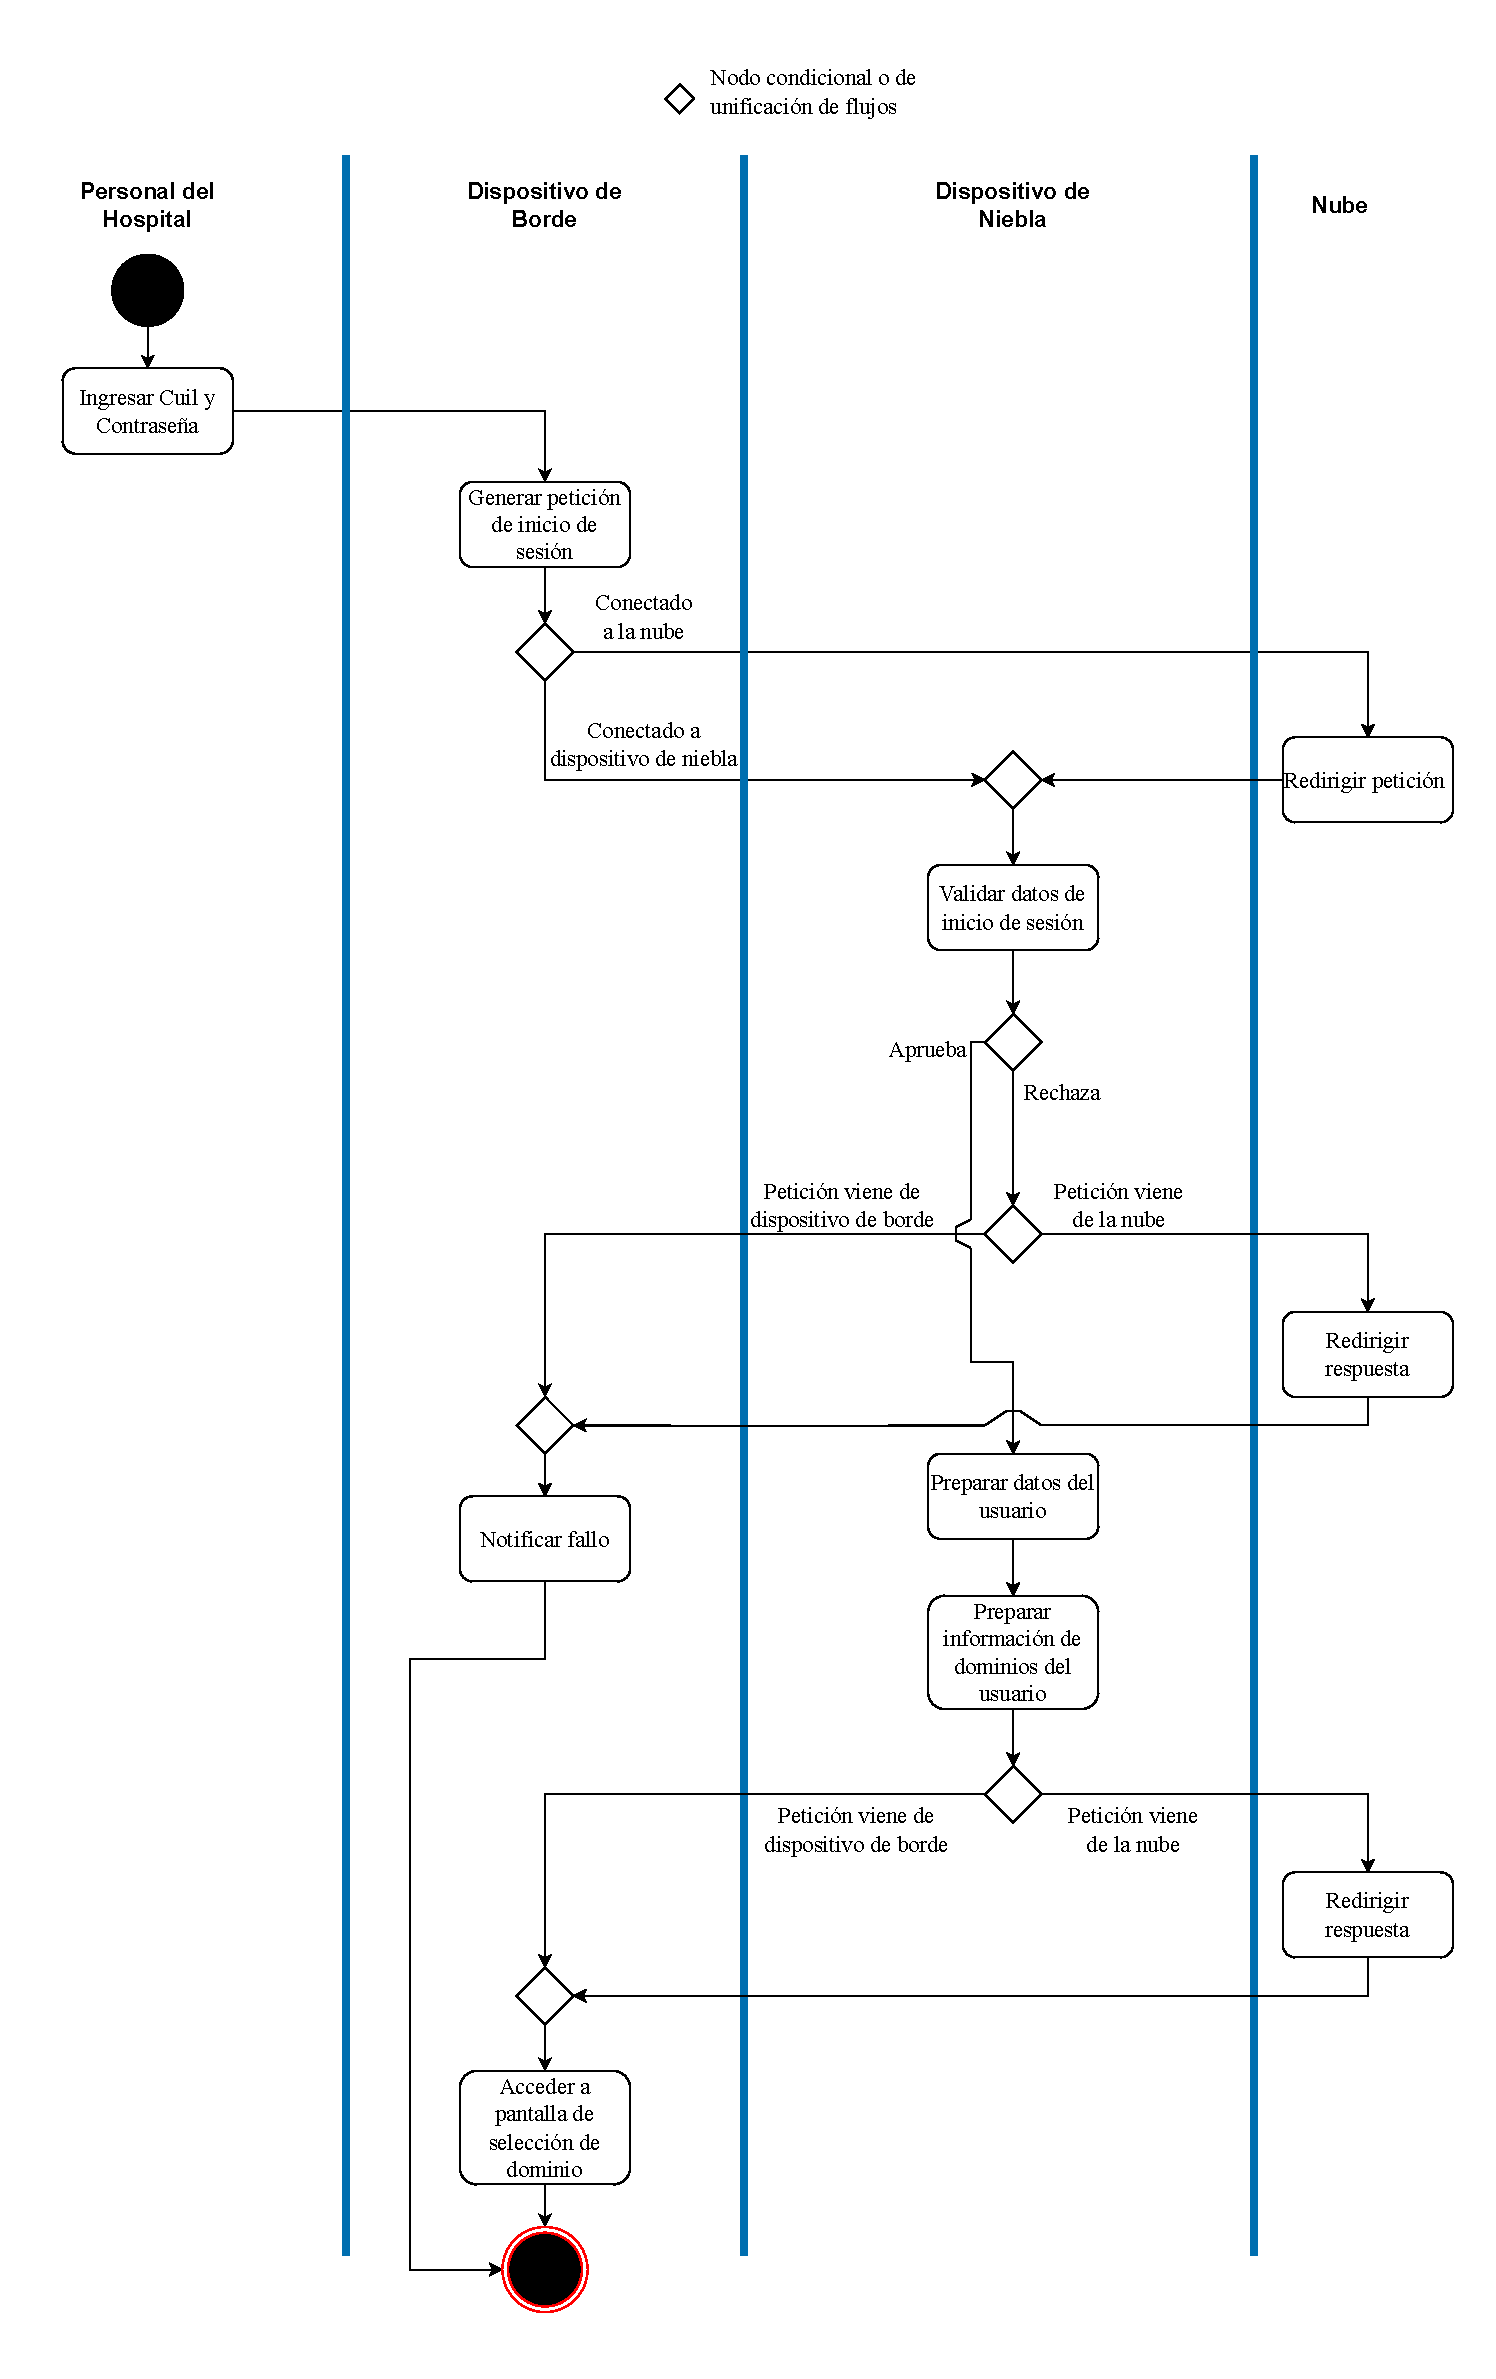
\includegraphics[height=\textheight, keepaspectratio]{Imagenes/Implementacion/IniciarSesionDA.pdf}
    \caption{Diagrama de actividades del caso de uso \textit{Iniciar Sesión}}
    \label{fig:diagActIniciarSesion}
\end{figure}




\begin{figure}
    \centering
    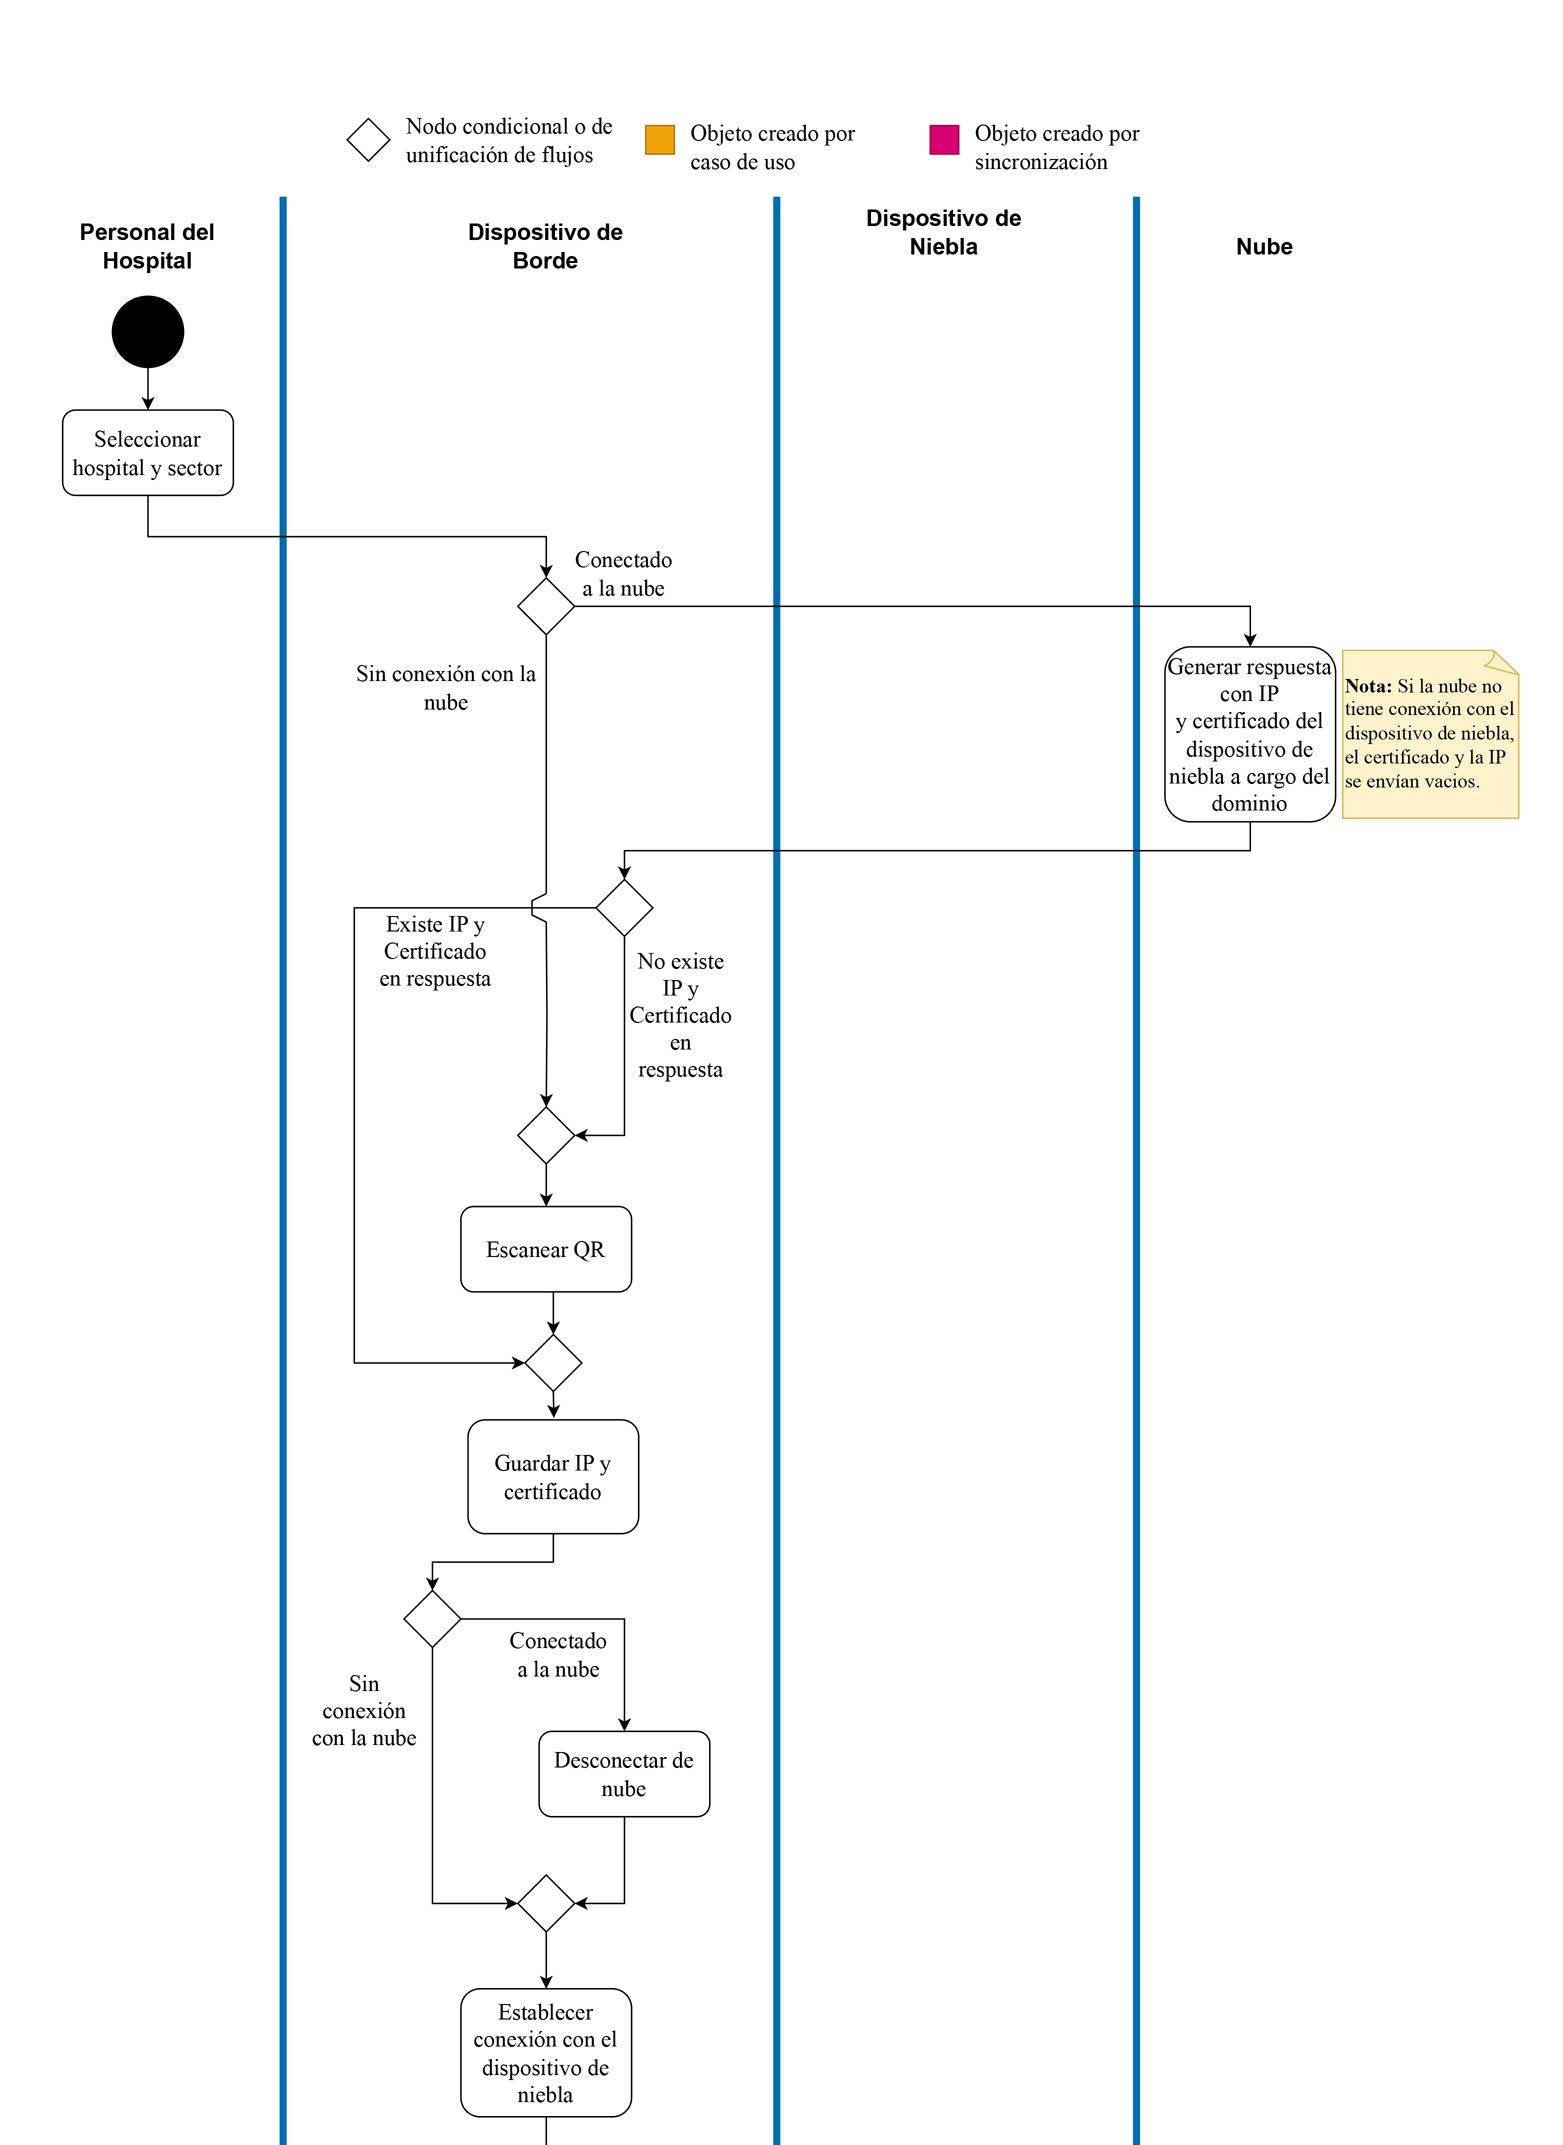
\includegraphics[width=\textwidth, height=\textheight, keepaspectratio]{Imagenes/Implementacion/ConectarseDominioDA1.pdf}
    \caption{Diagrama de actividades del caso de uso \textit{Conectarse a dominio} primer mitad}
    \label{fig:diagActConectDom}
\end{figure}

\begin{figure}
    \centering
    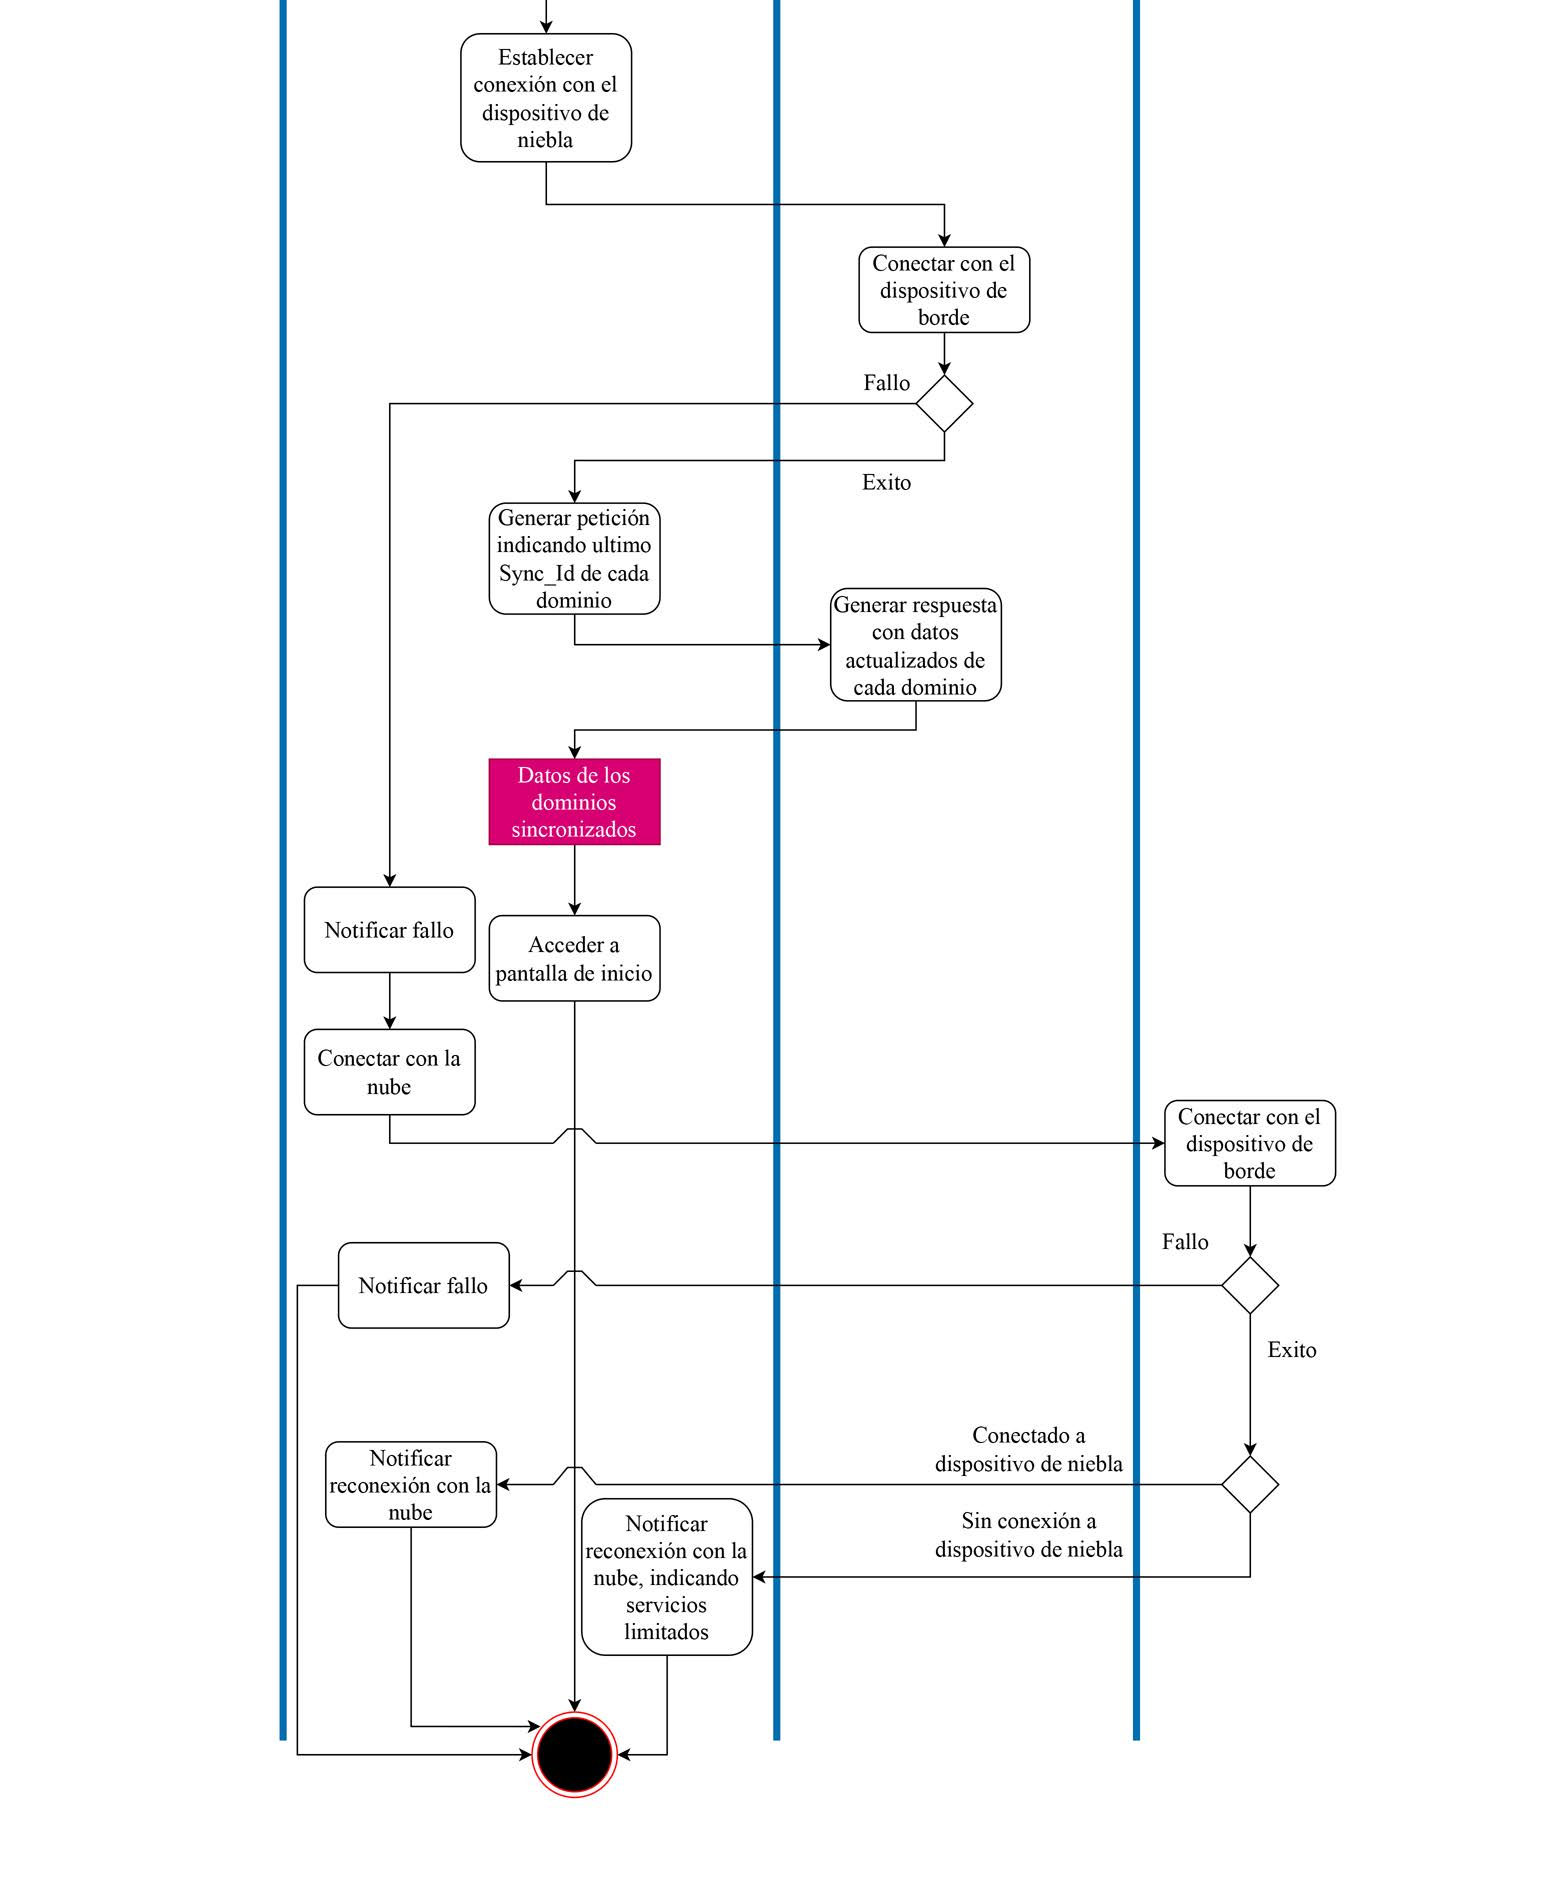
\includegraphics[width=\textwidth, height=\textheight, keepaspectratio]{Imagenes/Implementacion/ConectarseDominioDA2.pdf}
    \caption{Diagrama de actividades del caso de uso \textit{Conectarse a dominio} segunda mitad}
    \label{fig:diagActConectDom2}
\end{figure}

%\begin{figure}
%    \centering
    %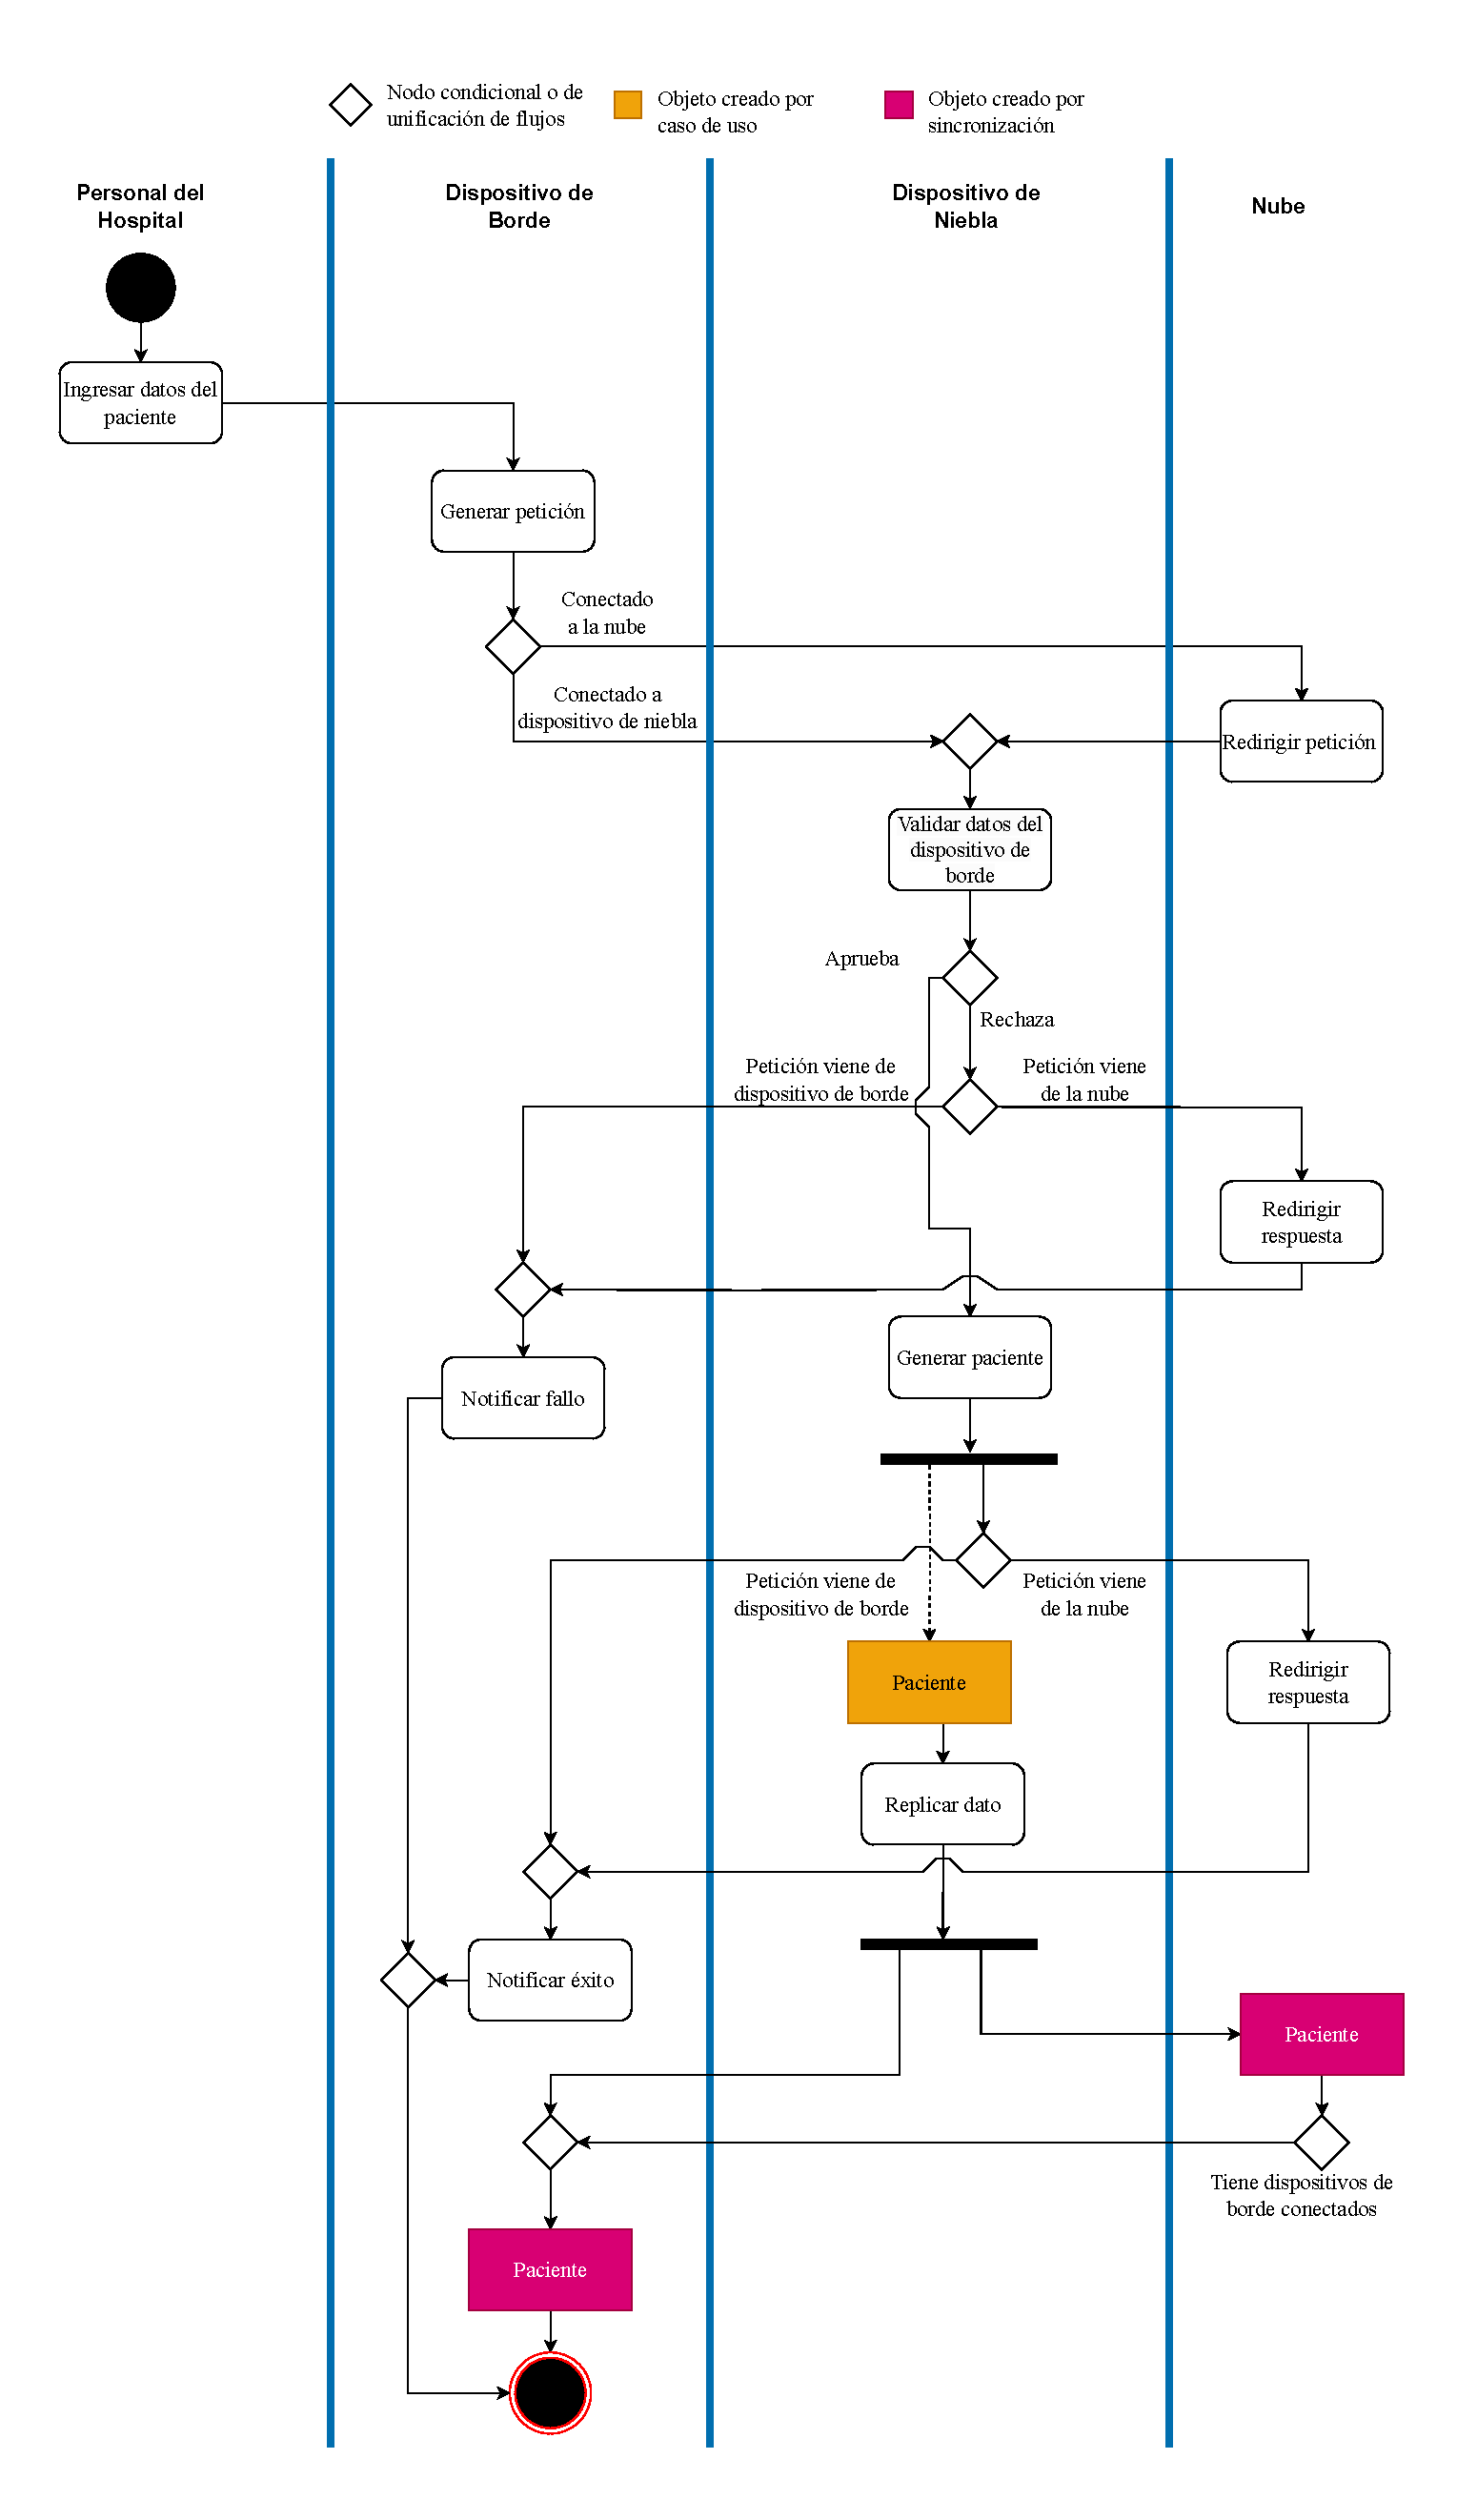
\includegraphics[width=\textwidth, height=\textheight, keepaspectratio]{Imagenes/Implementacion/IngresarPacienteDA.pdf}
    %\caption{Diagrama de actividades del caso de uso \textit{Admisión paciente}}
    %\label{fig:diagActIngresarPaciente}
%\end{figure}

\begin{figure}
    \centering
    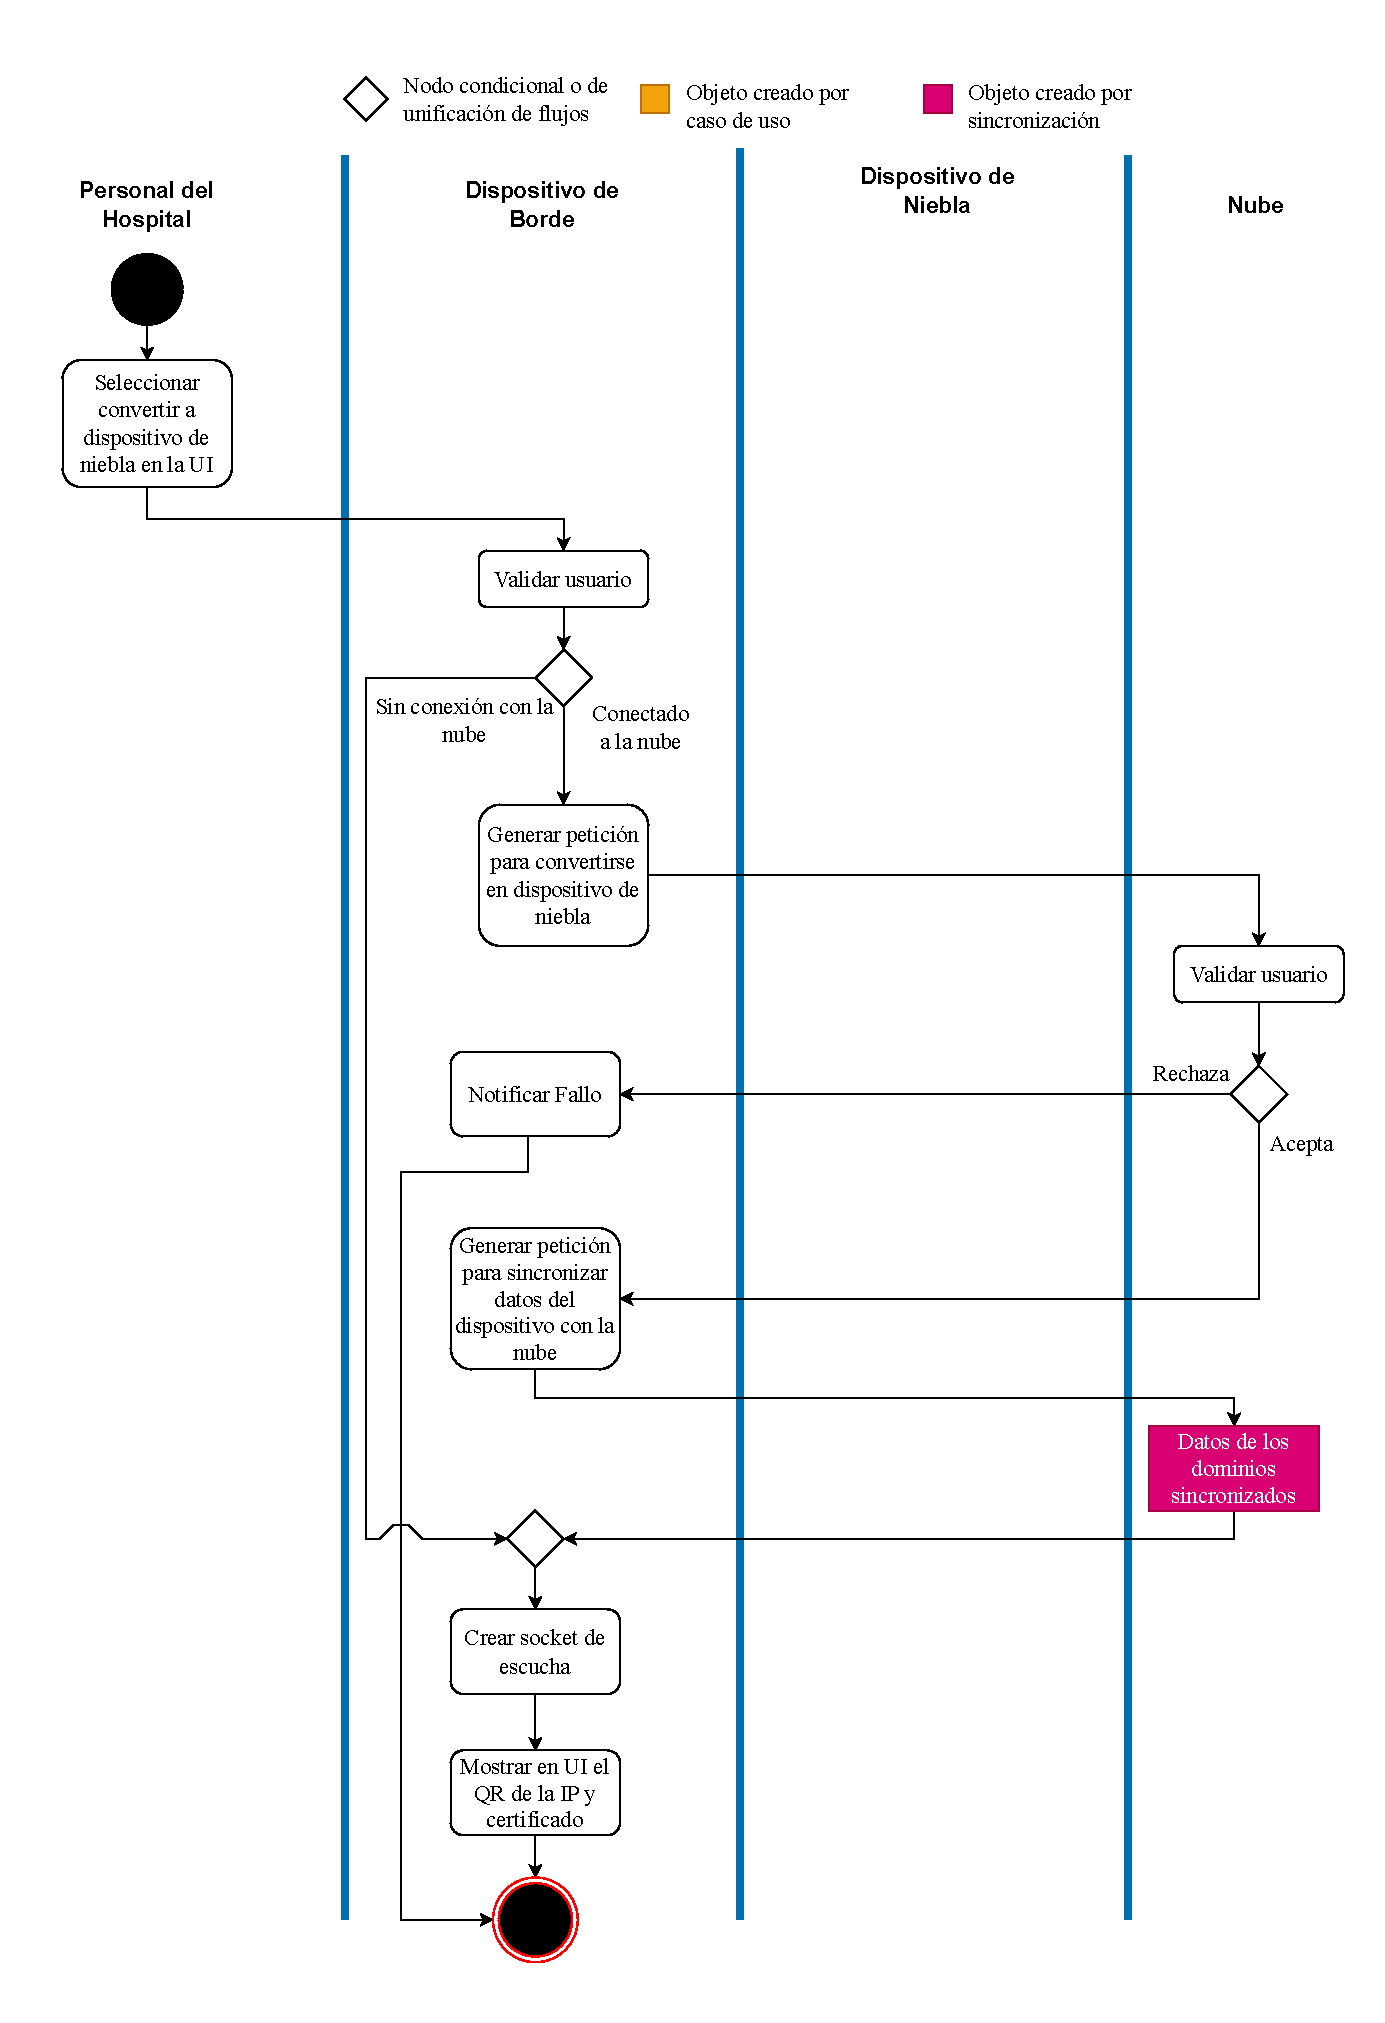
\includegraphics[width=\textwidth, height=\textheight, keepaspectratio]{Imagenes/Implementacion/ConvertirALiderDA.pdf}
    \caption{Diagrama de actividades del caso de uso \textit{Convertir a dispositivo de niebla}}
    \label{fig:diagActConvertALider}
\end{figure}


\chapter{Tabla de resultados de los experimentos}
\begin{table}[h]
\centering
\begin{tabular}{|l|p{4cm}|p{4cm}|c|}
\hline
\textbf{Cantidad de registros} & \textbf{Tamaño total requerido (bytes)} & \textbf{Tamaño real medido (bytes)} & \textbf{Sobrecarga \%} \\ \hline
100 & 13,600 & 188,416 & 1285.41\% \\ \hline
200 & 27,200 & 212,992 & 683.06\% \\ \hline
300 & 40,800 & 229,376 & 462.20\% \\ \hline
400 & 54,400 & 249,856 & 359.29\% \\ \hline
500 & 68,000 & 270,336 & 297.55\% \\ \hline
600 & 81,600 & 286,720 & 251.37\% \\ \hline
700 & 95,200 & 303,104 & 218.39\% \\ \hline
800 & 108,800 & 323,584 & 197.41\% \\ \hline
900 & 122,400 & 344,064 & 181.10\% \\ \hline
1000 & 136,000 & 364,544 & 168.05\% \\ \hline
1100 & 149,600 & 385,024 & 157.37\% \\ \hline
1200 & 163,200 & 397,312 & 143.45\% \\ \hline
1300 & 176,800 & 417,792 & 136.31\% \\ \hline
1400 & 190,400 & 438,272 & 130.18\% \\ \hline
1500 & 204,000 & 458,752 & 124.88\% \\ \hline
1600 & 217,600 & 475,136 & 118.35\% \\ \hline
1700 & 231,200 & 495,616 & 114.37\% \\ \hline
1800 & 244,800 & 516,096 & 110.82\% \\ \hline
1900 & 258,400 & 532,480 & 106.07\% \\ \hline
2000 & 272,000 & 552,960 & 103.29\% \\ \hline
2100 & 285,600 & 569,344 & 99.35\% \\ \hline
2200 & 299,200 & 589,824 & 97.13\% \\ \hline
2300 & 312,800 & 610,304 & 95.11\% \\ \hline
2400 & 326,400 & 630,784 & 93.25\% \\ \hline
2500 & 340,000 & 643,072 & 89.14\% \\ \hline
2600 & 353,600 & 663,552 & 87.66\% \\ \hline
2700 & 367,200 & 684,032 & 86.28\% \\ \hline
2800 & 380,800 & 704,512 & 85.01\% \\ \hline
2900 & 394,400 & 720,896 & 82.78\% \\ \hline
3000 & 408,000 & 741,376 & 81.71\% \\ \hline
\end{tabular}
\caption{Tamaño total requerido, tamaño real medido y sobrecarga de los registros (solo con registros tipo Paciente insertados)}
\label{tabla:TamReqYRealConOverPacientes}
\end{table}

\begin{table}[h]
\centering
\begin{tabular}{|l|p{4cm}|p{4cm}|c|}
\hline
\textbf{Cantidad de registros} & \textbf{Tamaño total requerido (bytes)} & \textbf{Tamaño real medido (bytes)} & \textbf{Sobrecarga \%} \\ \hline

3100 & 421,600 & 761,856 & 80.71\% \\ \hline
3200 & 435,200 & 778,240 & 78.82\% \\ \hline
3300 & 448,800 & 798,720 & 77.97\% \\ \hline
3400 & 462,400 & 815,104 & 76.28\% \\ \hline
3500 & 476,000 & 835,584 & 75.54\% \\ \hline
3600 & 489,600 & 856,064 & 74.85\% \\ \hline
3700 & 503,200 & 876,544 & 74.19\% \\ \hline
3800 & 516,800 & 888,832 & 71.99\% \\ \hline
3900 & 530,400 & 909,312 & 71.44\% \\ \hline
4000 & 544,000 & 929,792 & 70.92\% \\ \hline
4100 & 180,400 & 929,792 & 415.41\% \\ \hline
4200 & 184,800 & 946,176 & 412.00\% \\ \hline
4300 & 189,200 & 946,176 & 400.09\% \\ \hline
4400 & 193,600 & 954,368 & 392.96\% \\ \hline
4500 & 198,000 & 962,560 & 386.14\% \\ \hline
4600 & 202,400 & 978,944 & 383.67\% \\ \hline
4700 & 206,800 & 983,040 & 375.36\% \\ \hline
4800 & 211,200 & 991,232 & 369.33\% \\ \hline
4900 & 215,600 & 999,424 & 363.55\% \\ \hline
5000 & 220,000 & 1,007,616 & 358.01\% \\ \hline
5100 & 224,400 & 1,015,808 & 352.68\% \\ \hline
5200 & 228,800 & 1,028,096 & 349.34\% \\ \hline
5300 & 233,200 & 1,036,288 & 344.38\% \\ \hline
5400 & 237,600 & 1,044,480 & 339.60\% \\ \hline
5500 & 242,000 & 1,048,576 & 333.30\% \\ \hline
5600 & 246,400 & 1,056,768 & 328.88\% \\ \hline
5700 & 250,800 & 1,064,960 & 324.63\% \\ \hline
5800 & 255,200 & 1,069,056 & 318.91\% \\ \hline
5900 & 259,600 & 1,077,248 & 314.96\% \\ \hline
6000 & 264,000 & 1,081,344 & 309.60\% \\ \hline
\end{tabular}
\caption{Tamaño total requerido, tamaño real medido y sobrecarga de los registros (a los registros pacientes ingresados se le agregaron los registros Cama)}
\label{tabla:TamReqYRealConOverCamas}
\end{table}